\section{Preliminary Results}

\sepfootnotecontent{fn:impl}{ The algorithm implementation is available at the following link \newline
\href{https://github.com/constraintAutomaton/query-shape-detection}{https://github.com/constraintAutomaton/query-shape-detection}
and the integration in the Comunica query engine at the following link 
\href{https://github.com/constraintAutomaton/comunica-feature-link-traversal/tree/feature/shapeIndex}{https://github.com/constraintAutomaton/comunica-feature-link-traversal/tree/feature/shapeIndex}.
The implementation of the benchmark and complementary results such as the analysis of the statistical significance are available at the following link 
\href{https://github.com/constraintAutomaton/amw_shape_index_results}{https://github.com/constraintAutomaton/amw\_shape\_index\_results}.
}

\sepfootnotecontent{fn:ldp}{
  \href{https://www.w3.org/TR/ldp/}{https://www.w3.org/TR/ldp/}
}

\sepfootnotecontent{fn:propertyPath}{
  \href{https://www.w3.org/TR/sparql11-query/\#propertypaths}{https://www.w3.org/TR/sparql11-query/\#propertypaths}
}

An open-source implementation of the \href{https://github.com/constraintAutomaton/query-shape-detection}{algorithm} and an 
\href{https://github.com/constraintAutomaton/comunica-feature-link-traversal/tree/feature/shapeIndex}{integration} in the query engine 
Comunica \cite{taelman_iswc_resources_comunica_2018} is available online~\sepfootnote{fn:impl}.
We use the \href{https://github.com/SolidBench/SolidBench.js}{benchmark Solidbench} \cite{Taelman2023} to compare our approach with the current state-of-the-art (the \href{https://solid.github.io/type-indexes/}{type index} and the \href{https://www.w3.org/TR/ldp/}{LDP specification}~\sepfootnote{fn:ldp} as structural assumptions)~\cite{Taelman2023}.
We used the supported subset of SolidBench queries, skipping the currently unimplemented \href{https://www.w3.org/TR/sparql11-query/#propertypaths}{SPARQL property paths}~\sepfootnote{fn:propertyPath} and unions.
We executed each query 50 times with a timeout of 1 minute (6,000 ms).
Figure~\ref{fig:result} shows that the reduction can be as high as 80\% (D1V3 and S1V3) for execution time 
and 97\% (S1V3) for the number of HTTP requests.
Our approach reliably executes fewer HTTP requests compared to the state-of-the-art.
This is an expected result because no queries target (implicitly) each file of a user.
The shape index approach requests a subset of the request of the type index approach (without sacrificing query results) with the addition of the request to get the shape definitions which leads in general to the dereferencing of a small number of short documents.
There is not a direct correlation between the reduction of execution time and HTTP requests (e.g., the ratio 
between our approach and the state-of-the-art of the number of HTTP requests by the execution time for D1V3 is 0.5 compared to 0.15 for S1V3).
This hints at the results from the state-of-the-art \cite{Taelman2023} proposing that the query plan is the bottleneck for some queries in this environment,
however, the overhead of the containment calculation could also be a contributing factor to the current results.
In the worst cases, our approach  has similar query execution to the state-of-the-art except for D3V3 and D3V4 with an increase of 9\% of the mean of the execution time.
The variance of the execution with a shape index tends to be lower compared to the type index. 
A possible explanation for this observation is that the execution time of HTTP requests is unpredictable~\cite{hartig2016walking}
leading to an increase in variance.
This observation not only has potential implications for the reliability of multiple executions in terms of execution time
but also in terms of the performance of single executions in unstable networks where the server might take longer times to respond. 

\begin{figure}
  \centering
  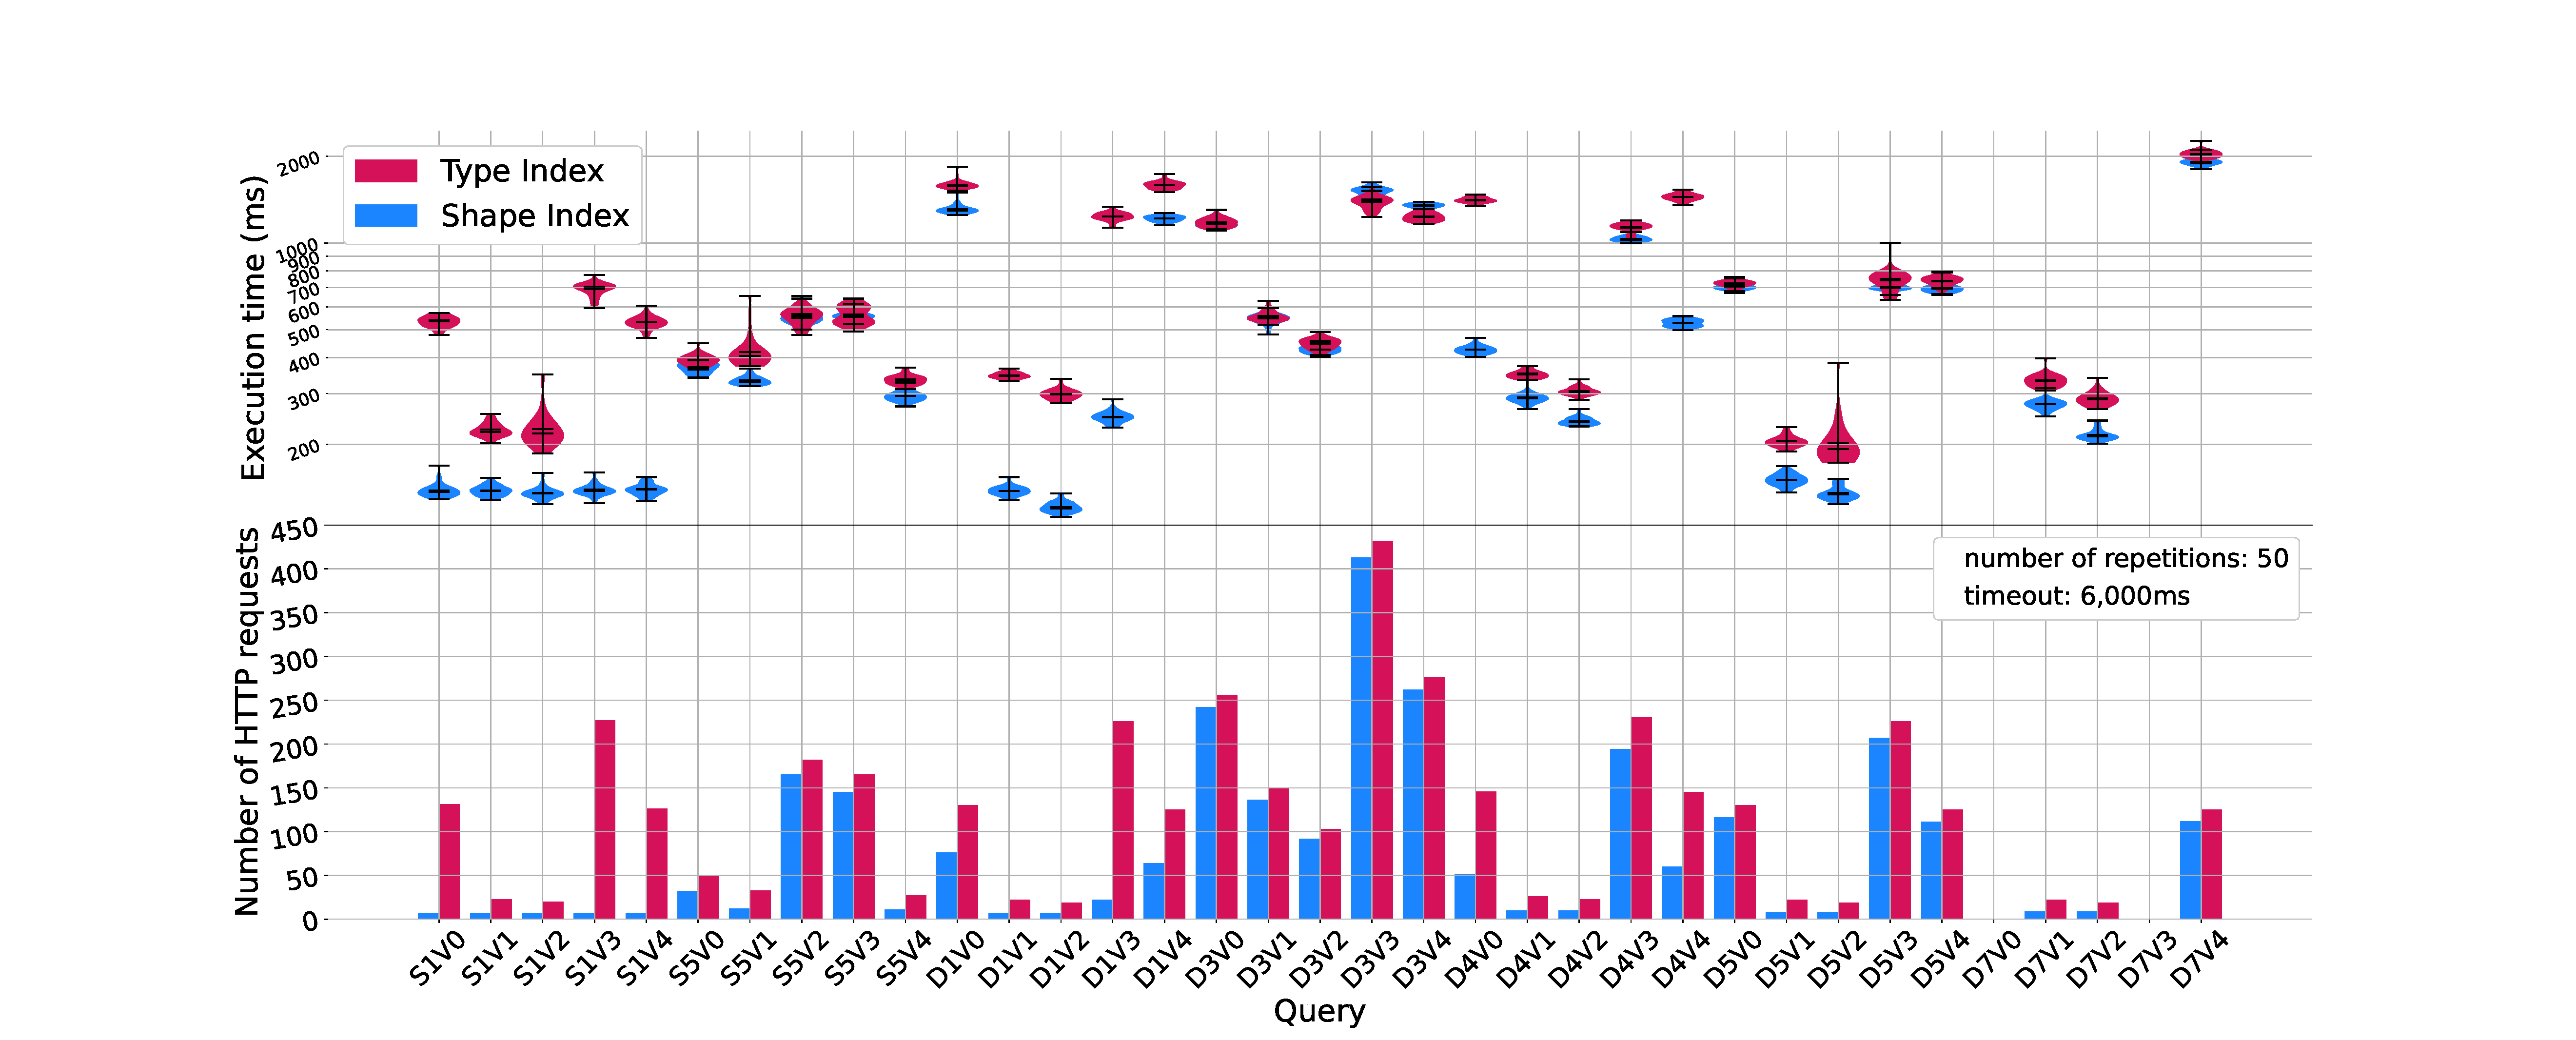
\includegraphics[width=\linewidth]{figure/combined}
  \caption{
  The execution time with shape indexes is consistently lower (up to 80\% with D1V3 and S1V3) or equal to that with the type indexes (except for D3V3 and D3V4), and always uses fewer HTTP requests.
  The queries are denoted with first the initial of the query template (e.g., S1 for interactive-\textbf{s}hort-\textbf{1}), and the version of the concrete query (e.g., V0). 
  Values not present in the plot (D7V0 and D7V3) indicate that the query timeout before the end of the execution.
  }
  \label{fig:result}
\end{figure}